%%%%%%%%%%%%%%%%%%%%%%%%%%%%%%%%%%%%%%%%%
% Beamer Presentation
% LaTeX Template
% Version 1.0 (10/11/12)
%
% This template has been downloaded from:
% http://www.LaTeXTemplates.com
%
% License:
% CC BY-NC-SA 3.0 (http://creativecommons.org/licenses/by-nc-sa/3.0/)
%
%%%%%%%%%%%%%%%%%%%%%%%%%%%%%%%%%%%%%%%%%

%----------------------------------------------------------------------------------------
%	PACKAGES AND THEMES
%----------------------------------------------------------------------------------------

\documentclass[xetex,mathserif,serif,14pt]{beamer}

\mode<presentation> {

% The Beamer class comes with a number of default slide themes
% which change the colors and layouts of slides. Below this is a list
% of all the themes, uncomment each in turn to see what they look like.

%\usetheme{default}
%\usetheme{AnnArbor}
%\usetheme{Antibes}
%\usetheme{Bergen}
%\usetheme{Berkeley}
%\usetheme{Berlin}
%\usetheme{Boadilla}
%\usetheme{CambridgeUS}
%\usetheme{Copenhagen}
%\usetheme{Darmstadt}
%\usetheme{Dresden}
%\usetheme{Frankfurt}
%\usetheme{Goettingen}
\usetheme[hideothersubsections]{Hannover}
%\usetheme{Ilmenau}
%\usetheme{JuanLesPins}
%\usetheme{Luebeck}
%\usetheme{Madrid}
%\usetheme{Malmoe}
%\usetheme{Marburg}
%\usetheme{Montpellier}
%\usetheme{PaloAlto}
%\usetheme{Pittsburgh}
%\usetheme{Rochester}
%\usetheme{Singapore}
%\usetheme{Szeged}
%\usetheme{Warsaw}

% As well as themes, the Beamer class has a number of color themes
% for any slide theme. Uncomment each of these in turn to see how it
% changes the colors of your current slide theme.

%\usecolortheme{albatross}
%\usecolortheme{beaver}
%\usecolortheme{beetle}
%\usecolortheme{crane}
\usecolortheme{dolphin}
%\usecolortheme{dove}
%\usecolortheme{fly}
%\usecolortheme{lily}
%\usecolortheme{orchid}
%\usecolortheme{rose}
%\usecolortheme{seagull}
%\usecolortheme{seahorse}
%\usecolortheme{whale}
%\usecolortheme{wolverine}
%\usecolortheme[named=magenta]{structure}

%\setbeamertemplate{footline} % To remove the footer line in all slides uncomment this line
%\setbeamertemplate{footline}[page number] % To replace the footer line in all slides with a simple slide count uncomment this line

%\setbeamercolor{frametitle}{fg=red,bg=red!20} % Redefine color of frame title box
%\setbeamercolor*{title}{bg=red,fg=white} % Redefine color of presentation title box
%\setbeamercolor{block title}{fg=black,bg=black!20} % Redefine color of block title %bg=background, fg=foreground
%\setbeamercolor{block body}{fg=black,bg=red!15} % Redefine color of block body

\makeatletter
\setbeamertemplate{footline} % Redefine footer (mainly width of boxes)
{
  \leavevmode%
  \hbox{%
  \begin{beamercolorbox}[wd=.41\paperwidth,ht=2.25ex,dp=1ex,center]{author in head/foot}%
    \usebeamerfont{author in head/foot}\insertshortauthor~~(\insertshortinstitute)
  \end{beamercolorbox}%
  \begin{beamercolorbox}[wd=.34\paperwidth,ht=2.25ex,dp=1ex,center]{title in head/foot}%
    \usebeamerfont{title in head/foot}\insertshorttitle
  \end{beamercolorbox}%
  \begin{beamercolorbox}[wd=.25\paperwidth,ht=2.25ex,dp=1ex,right]{date in head/foot}%
    \usebeamerfont{date in head/foot}\insertshortdate{}\hspace*{2em}
    \insertframenumber{} / \inserttotalframenumber\hspace*{2ex}
  \end{beamercolorbox}}%
  \vskip0pt%
}
\makeatother

\setbeamertemplate{navigation symbols}{} % To remove the navigation symbols from the bottom of all slides uncomment this line
}
\setbeamertemplate{caption}{\insertcaption}

\usepackage{polyglossia} % χρησιμοποιείται για καλύτερη υποστήριξη των Ελληνικών
\usepackage{graphicx} % Allows including images
\usepackage{booktabs} % Allows the use of \toprule, \midrule and \bottomrule in tables
\usepackage{pgfplots} % For drawing the queries
\usepgfplotslibrary{groupplots}
\usetikzlibrary{pgfplots.groupplots}
\usepackage{xcolor} % For colors
\usepackage[linesnumbered,vlined]{algorithm2e} % χρησιμοποιείται για τους αλγόριθμους
\usepackage{pgf-pie} % χρησιμοποιείται για πίτες

\pgfplotsset{compat=1.10}

\setmainlanguage[numerals=arabic]{greek} % κύρια γλώσσα
\setotherlanguages{english} % δευτερεύουσα γλώσσα

\SetAlFnt{\small}

%----------------------------------------------------------------------------------------
%	TITLE PAGE
%----------------------------------------------------------------------------------------

\title[Εξόντωση Σφηκών]{Εξόντωση Σφηκών με Χρήση Εξελικτικών Αλγορίθμων} % The short title appears at the bottom of every slide, the full title is only on the title page

\author[Χατσατριάν, Κοσματόπουλος]{Άνι Χατσατριάν, Μιχάλης Κοσματόπουλος} % Your name
\institute[ΑΤΕΙΘ] % Your institution as it will appear on the bottom of every slide, may be shorthand to save space
{
Αλεξάνδρειο Τεχνολογικό Εκπαιδευτικό Ίδρυμα Θεσσαλονίκης \\ % Your institution for the title page
\medskip
\textit{\{achatsat, mkosm\}@it.teithe.gr} % Your email address
}
\titlegraphic{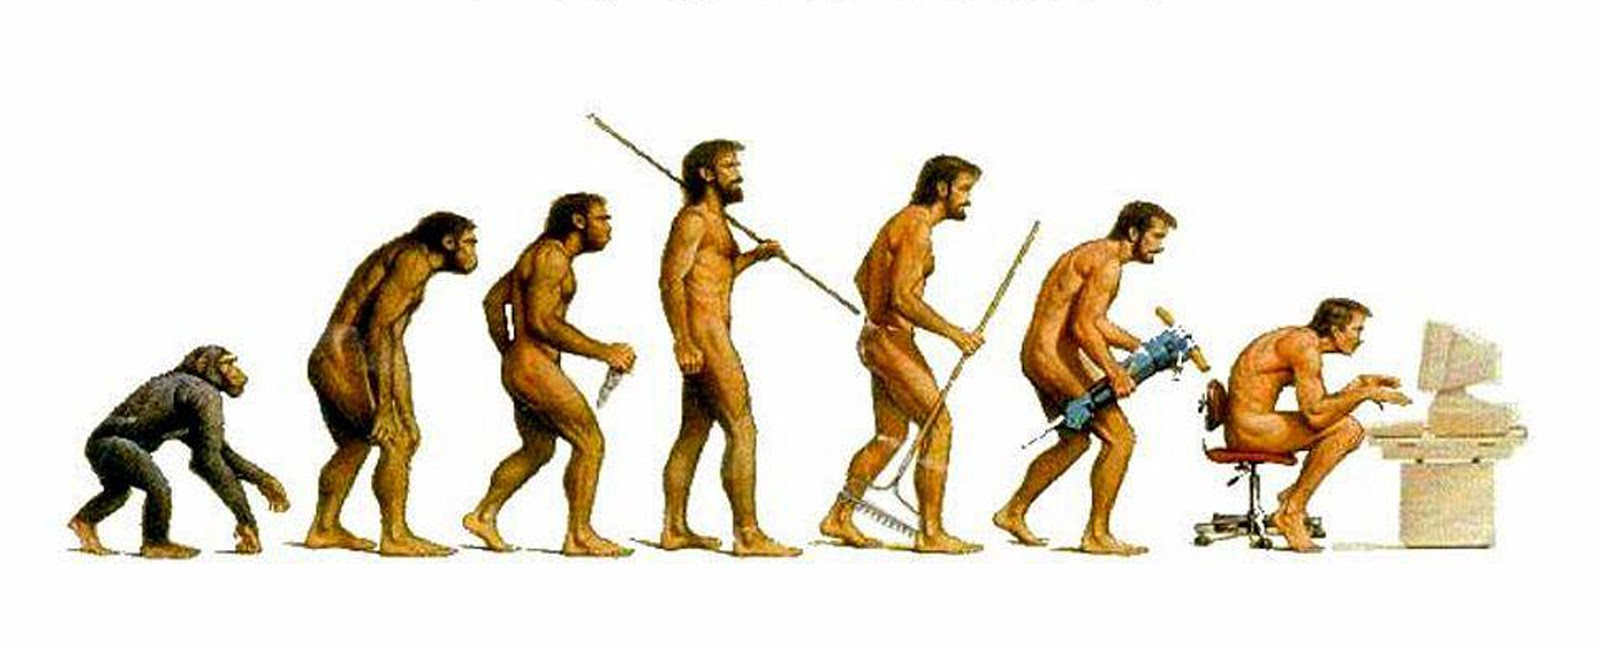
\includegraphics[height=2.3cm]{images/evolution.jpg} }
\date{23 Μαΐου 2014} % Date, can be changed to a custom date

\newfontfamily\greekfont[Script=Greek]{Linux Libertine O} % work-around για bug του polyglossia
\setmainfont[Kerning=On,Mapping=tex-text]{Linux Libertine O} % roman font

\begin{document}

\begin{frame}
\titlepage % Print the title page as the first slide
\end{frame}

%\begin{frame}
%\frametitle{Overview} % Table of contents slide, comment this block out to remove it
%\tableofcontents % Throughout your presentation, if you choose to use \section{} and \subsection{} commands, these will automatically be printed on this slide as an overview of your presentation
%\end{frame}

%----------------------------------------------------------------------------------------
%	PRESENTATION SLIDES
%----------------------------------------------------------------------------------------

%------------------------------------------------
\section{Εισαγωγή} % Sections can be created in order to organize your presentation into discrete blocks, all sections and subsections are automatically printed in the table of contents as an overview of the talk
%------------------------------------------------

\begin{frame}
\frametitle{Εισαγωγή}
Στόχος της εργασίας είναι η εύρεση της βέλτιστης λύσης ενός προβλήματος με τη χρήση ενός εξελικτικού αλγορίθμου.

\end{frame}

\section{Βιολογικό Υπόβαθρο}

\subsection{Η Θεωρία της Εξέλιξης}

\begin{frame}

\frametitle{Η Θεωρία της Εξέλιξης}
\begin{tikzpicture}[remember picture,overlay]
\node[anchor=north west,xshift=75pt] at (current page.north west) {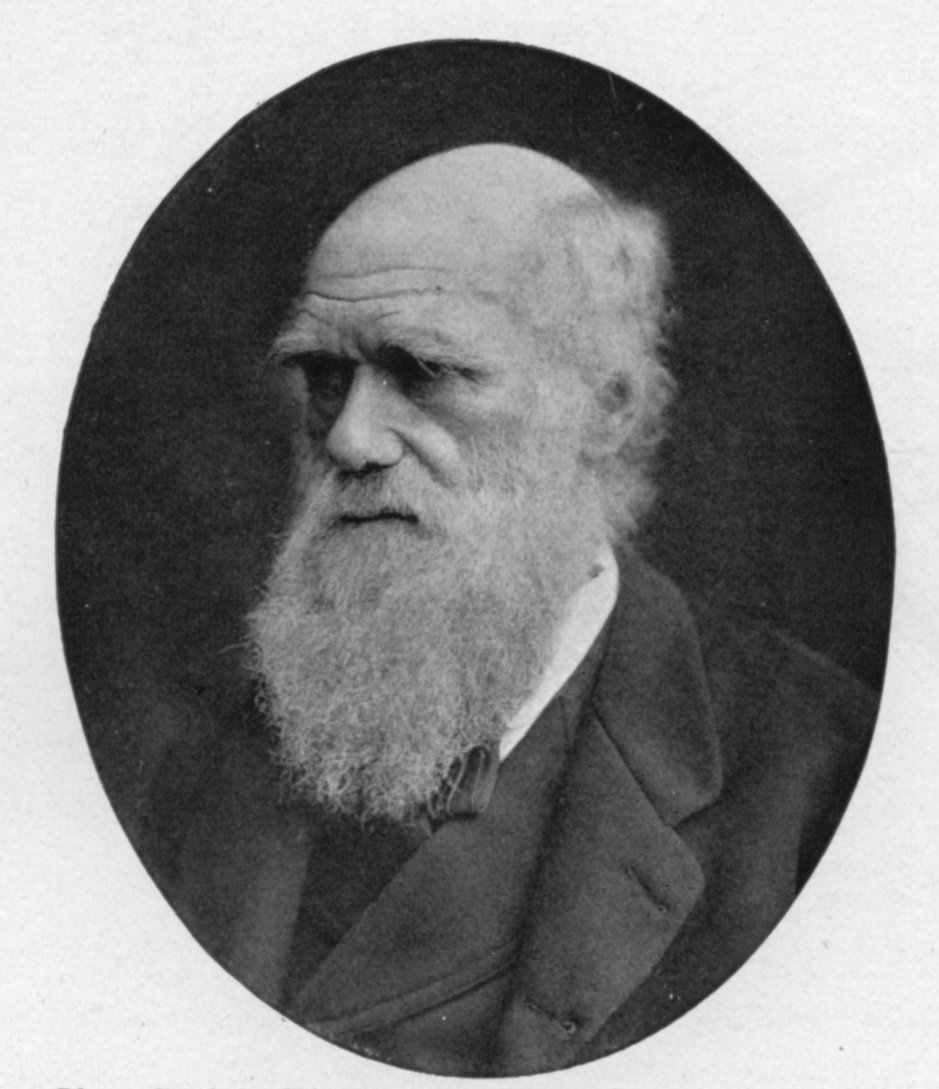
\includegraphics[height=3cm]{images/charles2.jpg}};
\end{tikzpicture}
\begin{itemize}
  \item Η ικανότητα των οργανισμών να προσαρμόζονται στις αλλαγές του περιβάλλοντος και να αποκτούν απογόνους.\pause
  \item Οι αποκλίσεις στους φαινότυπους των οργανισμών.
\end{itemize}
\end{frame}

\subsection{Βιολογικά Χαρακτηριστικά}

\begin{frame}
\frametitle{Βιολογικά Χαρακτηριστικά}
\begin{tikzpicture}[remember picture,overlay]
\node[anchor=north east,yshift=-120pt, xshift=-40] at (current page.north east) {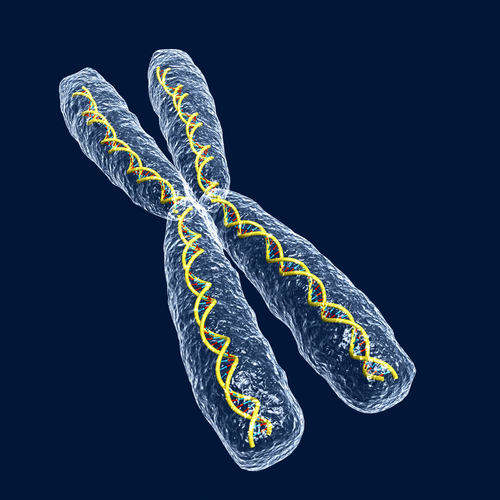
\includegraphics[height=3cm]{images/chromo.jpg}};
\end{tikzpicture}
    \begin{itemize}
      \item Γονίδια\pause
      \item Alleles\pause
      \item Χρωμόσωμα\pause
      \item Γονότυπος\pause
      \item Φαινότυπος
    \end{itemize}
\end{frame}

\section{Μοντέλα Εξελικτικών Αλγορίθμων}

\subsection{Γενική μορφή ΕΑ}

\begin{frame}
\frametitle{Γενική μορφή ΕΑ}
\centering
\begin{algorithm}[H]
    $population \gets randomPopulation(populationSize)$\;
    $evolutions \gets 0$\;
    \While{$evolutions < maxEvolutions$}{
        $parents \gets selectParents(population)$\;
        $population \gets recombine(parents)$\;
        $population \gets mutate(population)$\;
        $evolutions \gets evolutions + 1$\;
    }
    \Return{$getBestChromosome(population)$}\;
\end{algorithm}
%\begin{enumerate}
%  \item Δημιουργία πληθυσμού
%  \item Επιλογή γονέων
%  \item Ανασυνδυασμός γονέων
%  \item Μετάλλαξη γονέων
%  \item
%\end{enumerate}
\end{frame}

\subsection{Γενετικοί Αλγόριθμοι}

\begin{frame}
\frametitle{Γενετικοί Αλγόριθμοι}
\begin{itemize}
  \item «Γεννήθηκαν» την δεκαετία του '60 από τον John Holland\pause
  \item Είναι μια κλάση από αλγορίθμους αναζήτησης, βασισμένοι στη βιολογική εξέλιξη\pause
  \item Ακολουθούν μια επαναληπτική διαδικασία, και κάθε επανάληψη ονομάζεται γενιά
\end{itemize}
\end{frame}

\subsection{Τρόποι Αναπαράστασης}

\begin{frame}
\frametitle{Τρόποι Αναπαράστασης}
\begin{itemize}
  \item Πιο συνηθισμένος τρόπος αναπαράστασης: bit string
  \begin{figure}
    \renewcommand{\arraystretch}{1.3}
    \label{fig_bit_string}
    \centering
    \begin{tabular}{c|c|c|c|c|c|c|c}
        \hline
        \ldots & 0 & 0 & 1 & 0 & 1 & 1 & \ldots\\
        \hline
    \end{tabular}
    \caption{Παράδειγμα bit string}
  \end{figure}
  \item Μεταθέσεις
  \item Δεντρική δομή
\end{itemize}
\end{frame}

\subsection{Δημιουργία και Αξιολόγηση Πληθυσμού}

\begin{frame}
\frametitle{Δημιουργία και Αξιολόγηση Πληθυσμού}
\begin{itemize}
  \item Δημιουργούνται $N$ τυχαία σταθερού-μήκους bit string
  \item Η αξιολόγηση γίνεται με τη συνάρτηση καταλληλότητας
\end{itemize}
\end{frame}

\subsection{Επιλογή Γονέων}

\begin{frame}
\frametitle{Επιλογή Γονέων}
\begin{itemize}
  \item Μετά την αξιολόγηση, πρέπει να επιλεχθούν τα χρωμοσώματα που θα γίνουν γονείς.
  \item Τα χρωμοσώματα που δίνουν καλύτερη λύση στο πρόβλημα πρέπει να έχουν περισσότερες πιθανότητες να επιλεχθούν
  \item Υπάρχουν διάφορες τεχνικές για την επιλογή
\end{itemize}
\end{frame}

\subsubsection*{Επιλογή Ρουλέτας}

\begin{frame}
\frametitle{Επιλογή Ρουλέτας}
\begin{tiny}
\begin{table}
    \centering
    \begin{tabular}{@{}crrrr@{}}
        \toprule
        Α/Α Χρωμοσώματος & Καταλληλότητα & Συνολικό ποσοστό & Κατάταξη & Ποσοστό κατάταξης \\ \midrule
        1                & 40            & 14.8\%           & 4        & 19\%              \\
        2                & 110           & 40.7\%           & 6        & 28.5\%            \\
        3                & 30            & 11.1\%           & 3        & 14.3\%            \\
        4                & 25            & 9.3\%            & 2        & 9.6\%             \\
        5                & 45            & 16.7\%           & 5        & 23.8\%            \\
        6                & 20            & 7.4\%            & 1        & 4.8\%             \\ \midrule
        Σύνολο           & 270           & 100\%            &          & 100\%             \\ \bottomrule
    \end{tabular}
    \caption{Πληθυσμός}
\end{table}
\begin{figure}
    \centering
    \begin{tikzpicture}
        \pie[rotate=45, radius=1]{14.8/1, 7.4/6, 16.7/5, 9.3/4, 11.1/3, 40.7/2}
    \end{tikzpicture}
    \begin{tikzpicture}
        \pie[rotate=45, radius=1]{19/1, 4.8/6, 23.8/5, 9.6/4, 14.3/3, 28.5/2}
    \end{tikzpicture}

    \caption{Ποσοστά καταλληλότητας και κατάταξης}
\end{figure}
\end{tiny}
\end{frame}

\subsubsection*{Επιλογή Τουρνουά}

\begin{frame}
\frametitle{Επιλογή Τουρνουά}
\begin{itemize}
  \item Δημιουργία ενός τυχαίου υποσυνόλου k από τον αρχικό πληθυσμό.\pause
  \item Επιλογή του καλύτερου χρωμοσώματος από αυτό το υποσύνολο (pool).
\end{itemize}
\end{frame}

\subsubsection*{Ελιτισμός}

\begin{frame}
\frametitle{Ελιτισμός}
Tα άτομα με την μεγαλύτερη καταλληλότητα συνεχίζουν στην επόμενη γενιά χωρίς να υποστούν καμία αλλαγή.
\end{frame}

\subsection{Αναπαραγωγή των Γονέων}

\begin{frame}
\frametitle{Αναπαραγωγή των Γονέων}
Μετά την επιλογή, θα πρέπει να εφαρμοστεί ένας ή περισσότεροι τελεστές για τη δημιουργία των χρωμοσωμάτων-παιδιών
\end{frame}

\subsubsection{Διασταύρωση Ενός Σημείου}

\begin{frame}
\frametitle{Διασταύρωση Ενός Σημείου}
\begin{figure}[!t]
    \centering
    \def\svgwidth{3.2in}
    \input{./images/OnePointCrossover.pdf_tex}
    \caption{Διασταύρωση ενός σημείου}
    \label{fig_opc}
\end{figure}
\end{frame}

\subsubsection{Διασταύρωση Δύο Σημείων}

\begin{frame}
\frametitle{Διασταύρωση Δύο Σημείων}
\begin{figure}[!t]
    \centering
    \def\svgwidth{3.2in}
    \input{./images/TwoPointCrossover.pdf_tex}
    \caption{Διασταύρωση δύο σημείων}
    \label{fig_tpc}
\end{figure}
\end{frame}

\subsubsection{Μετάλλαξη}

\begin{frame}
\frametitle{Μετάλλαξη}
Επιλέγεται τυχαία ένα bit από το χρωμόσωμα, και αυτό αντιστρέφεται.

\begin{figure}
    \begin{tabular}{|c|c|c|c|}
        \hline
        1 & 0 & 0 & 0\\
        \hline
    \end{tabular}
    \begin{tabular}{|c|c|c|c|}
        \hline
        1 & 0 & 1 & 0\\
        \hline
    \end{tabular}
    \caption{Μετάλλαξη ενός χρωμοσώματος}
    \label{fig_mutation}
\end{figure}
\end{frame}

\subsection{Παράλληλοι Γενετικοί Αλγόριθμοι}

\begin{frame}
\frametitle{Παράλληλοι Γενετικοί Αλγόριθμοι}
\begin{itemize}
  \item Coarse Grain
  \item Fine Grain
\end{itemize}
\end{frame}

\subsection{Εξελικτικές Στρατηγικές}

\begin{frame}
\frametitle{Εξελικτικές Στρατηγικές}
\begin{itemize}
  \item Προτάθηκαν στις αρχές του '60 από τους Ingo Rechenberg και Hans-Paul Schewefel.
  \item Αφορούν την επίλυση τεχνικών προβλημάτων βελτιστοποίησης.
  \item Χρησιμοποιούν μόνο τελεστές μετάλλαξης.
  \item Στην απλή της μορφή κάθε γονέας δημιουργεί έναν απόγονο για κάθε γενιά.
\end{itemize}
\end{frame}

\subsection{Γενετικός Προγραμματισμός}

\begin{frame}
\frametitle{Γενετικός Προγραμματισμός}
\begin{itemize}
  \item Αναζήτηση του αλγορίθμου που αρμόζει στην επίλυση ενός προβλήματος.
  \item Εξέλιξη του αλγορίθμου που λύνει το πρόβλημα.
  \item Σημαντική ενίσχυση από τον John Koza το '90.
  \item Προγράμματα == Δεδομένα.
  \item Εφαρμογή τελεστών διασταύρωσης και μετάλλαξης.
\end{itemize}
\end{frame}

%------------------------------------------------

\section{Παρουσίαση του προβλήματος}

\begin{frame}
\frametitle{Παρουσίαση του προβλήματος}
\begin{figure}[!t]
    \centering
    \begin{tikzpicture}
    	\begin{axis}[
            xlabel={x},
            ylabel={y},
            width = 0.6\columnwidth,
            %height = 0.8\columnwidth,
            colorbar,
            legend cell align = left,
            legend pos = north west,
            %colormap = {whiteblack}{gray(0cm) = (1); gray(1cm) = (0)},
            colorbar style = {title=Αριθμός Σφηκών, /tikz/.cd},
            font = \footnotesize]

            \addplot +[scatter, only marks, point meta=explicit] table [meta=wasps, col sep=comma] {../figures/waspNests.csv};
            \addlegendentry{Σφηκοφωλιά}
        \end{axis}
    \end{tikzpicture}
    \caption{Χάρτης σφηκοφωλιών}
    \label{fig_waspNestsMap}
\end{figure}
\end{frame}

%------------------------------------------------

\section{Επίλυση}

\subsection{JGAP}

\begin{frame}
\frametitle{Βήματα υλοποίησης}
\begin{enumerate}
  \item Σχεδιασμός χρωμοσώματος\pause
  \item Υλοποίηση συνάρτησης καταλληλότητας\pause
  \item Ορισμός των παραμέτρων\pause
  \item Δημιουργία ενός πληθυσμού από υποψήφιες λύσεις\pause
  \item Εξέλιξη του πληθυσμού
\end{enumerate}
\end{frame}

\subsection{Ανάλυση Προβλήματος}

\begin{frame}
\frametitle{Ανάλυση Προβλήματος}
\begin{itemize}
  \item Πρόβλημα μεγιστοποίησης -> Αύξηση αριθμού εξοντωμένων σφηκών
  \item Πρόβλημα ελαχιστοποίησης -> Μείωση του αριθμού των σφηκών που απομένουν στη σοφίτα
\end{itemize}
\end{frame}

\subsection{Περιγραφή Λύσης}

\begin{frame}
\frametitle{Περιγραφή Λύσης}
\begin{figure}[!t]
    \centering
    \begin{tabular}{|c|c|c|c|c|c|}
        \hline
        $x_1$ & $y_1$ & $x_2$ & $y_2$ & $x_3$ & $y_3$\\
        \hline
    \end{tabular}
    \caption{Δομή χρωμοσώματος}
    \label{fig_chromosomeStructure}
\end{figure}
\end{frame}

\subsection{Σύγκριση Αποτελεσμάτων}

\subsubsection{Σύγκριση με τη Βέλτιστη Λύση}
\begin{frame}
\frametitle{Σύγκριση με τη Βέλτιστη Λύση}

\end{frame}

\subsubsection{Σύγκριση Μεθόδου Επιλογής}
\begin{frame}
\frametitle{Σύγκριση Μεθόδου Επιλογής}
 \centering
    \begin{tikzpicture}
        \begin{axis}[
            scale=0.8,
            xlabel={Αριθμός γενιάς},
            ylabel={Καταλληλότητα},
            %ymin = 2300,
            legend cell align = left,
            legend pos = south east,
            font = \footnotesize]

            \addplot +[mark=none] table [x=gen, y=pop20, col sep=comma] {../figures/averageFitness.csv};
            \addlegendentry{πληθ. = 20}
            \addplot +[mark=none] table [x=gen, y=pop50, col sep=comma] {../figures/averageFitness.csv};
            \addlegendentry{πληθ. = 50}
            \addplot +[mark=none] table [x=gen, y=pop100, col sep=comma] {../figures/averageFitness.csv};
            \addlegendentry{πληθ. = 100}
            \addplot +[mark=none] table [x=gen, y=pop1000, col sep=comma] {../figures/averageFitness.csv};
            \addlegendentry{πληθ. = 1000}
        \end{axis}
    \end{tikzpicture}
\end{frame}

\subsubsection{Σύγκριση Μεγέθους Πληθυσμού}

\begin{frame}
\frametitle{Σύγκριση Μεγέθους Πληθυσμού}
\centering
 \begin{tikzpicture}
        \begin{axis}[
            scale=0.8,
            xlabel={Αριθμός γενιάς},
            ylabel={Καταλληλότητα},
            %ymin = 2300,
            legend cell align = left,
            legend pos = south east,
            font = \footnotesize]
            \addplot +[mark=none] table [x=gen, y=bestchrom, col sep=comma] {../figures/selectors.csv};
            \addlegendentry{BestChromosomesSelector}
            \addplot +[mark=none] table [x=gen, y=roulette, col sep=comma] {../figures/selectors.csv};
            \addlegendentry{WeightedRouletteSelector}
            \addplot +[mark=none] table [x=gen, y=tournament, col sep=comma] {../figures/selectors.csv};
            \addlegendentry{TournamentSelector}
        \end{axis}
    \end{tikzpicture}
\end{frame}

\subsubsection{Σύγκριση βάσει ποσοστού ανασυνδυασμού}

\begin{frame}
\frametitle{Σύγκριση βάσει ποσοστού ανασυνδυασμού}
\centering
    \begin{tikzpicture}
        \begin{axis}[
            scale=0.8,
            xlabel={Πιθανότητα ανασυνδυασμού},
            ylabel={Καταλληλότητα},
            ymin = 2000,
            legend cell align = left,
            legend pos = south east,
            font = \footnotesize]

            \addplot +[mark=none] table [x=a, y=b, col sep=comma] {../figures/crossoverRateFitness.csv};
            \addlegendentry{πληθ. = 50, γεν. = 5}
            \addplot +[mark=none] table [x=a, y=c, col sep=comma] {../figures/crossoverRateFitness.csv};
            \addlegendentry{πληθ. = 50, γεν. = 10}
            \addplot +[mark=none] table [x=a, y=d, col sep=comma] {../figures/crossoverRateFitness.csv};
            \addlegendentry{πληθ. = 20, γεν. = 5}
            \addplot +[mark=none] table [x=a, y=e, col sep=comma] {../figures/crossoverRateFitness.csv};
            \addlegendentry{πληθ. = 20, γεν. = 10}
        \end{axis}
    \end{tikzpicture}
\end{frame}

\section{Συμπέρασμα}

\begin{frame}
\frametitle{Συμπέρασμα}
\begin{itemize}
  \item Γρήγορη επίλυση πολύπλοκων προβλημάτων\pause
  \item Μεγάλη προσαρμοστικότητα\pause
  \item Χώρος για βελτίωση
\end{itemize}
\end{frame}


\begin{frame}

\Huge{\centerline{Thank You}}
\Large{\centerline{Questions?}}
\end{frame}

%----------------------------------------------------------------------------------------

\end{document} 